\documentclass{article}
\usepackage[utf8]{inputenc}

\usepackage{amssymb}
\usepackage{amsmath}

\title{Time Series Project 1}
\author{Stefan Eng }
\date{April 2019}

\usepackage{natbib}
\usepackage{graphicx}

\begin{document}

\maketitle

\section{Introduction}
\cite{bd}

\section*{Problem 1}
mean correct all three series, i.e., subtract the sample mean from each series.

\begin{figure}[t]
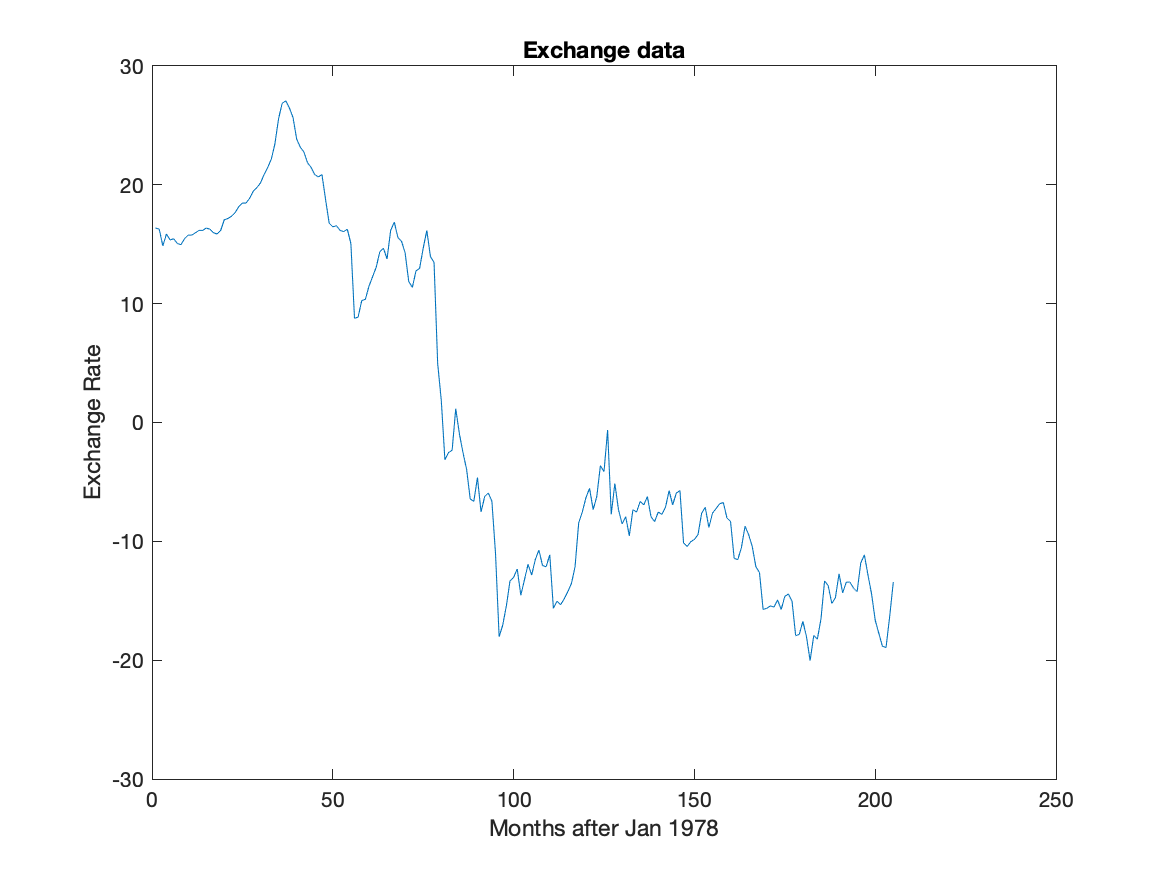
\includegraphics[width=8cm]{plots/exchangedata.png}
\centering
\end{figure}

\begin{figure}[t]
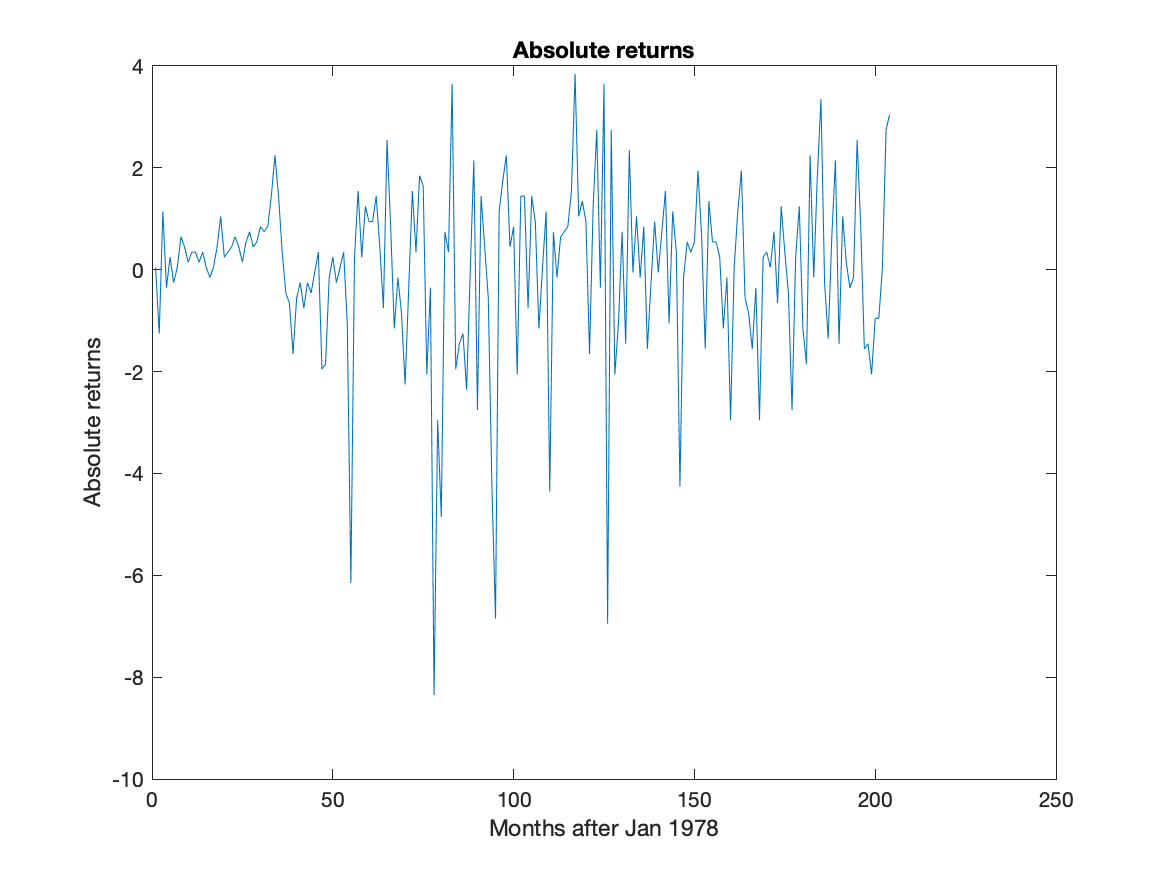
\includegraphics[width=8cm]{plots/abs_returns.png}
\centering
\end{figure}

\begin{figure}[t]
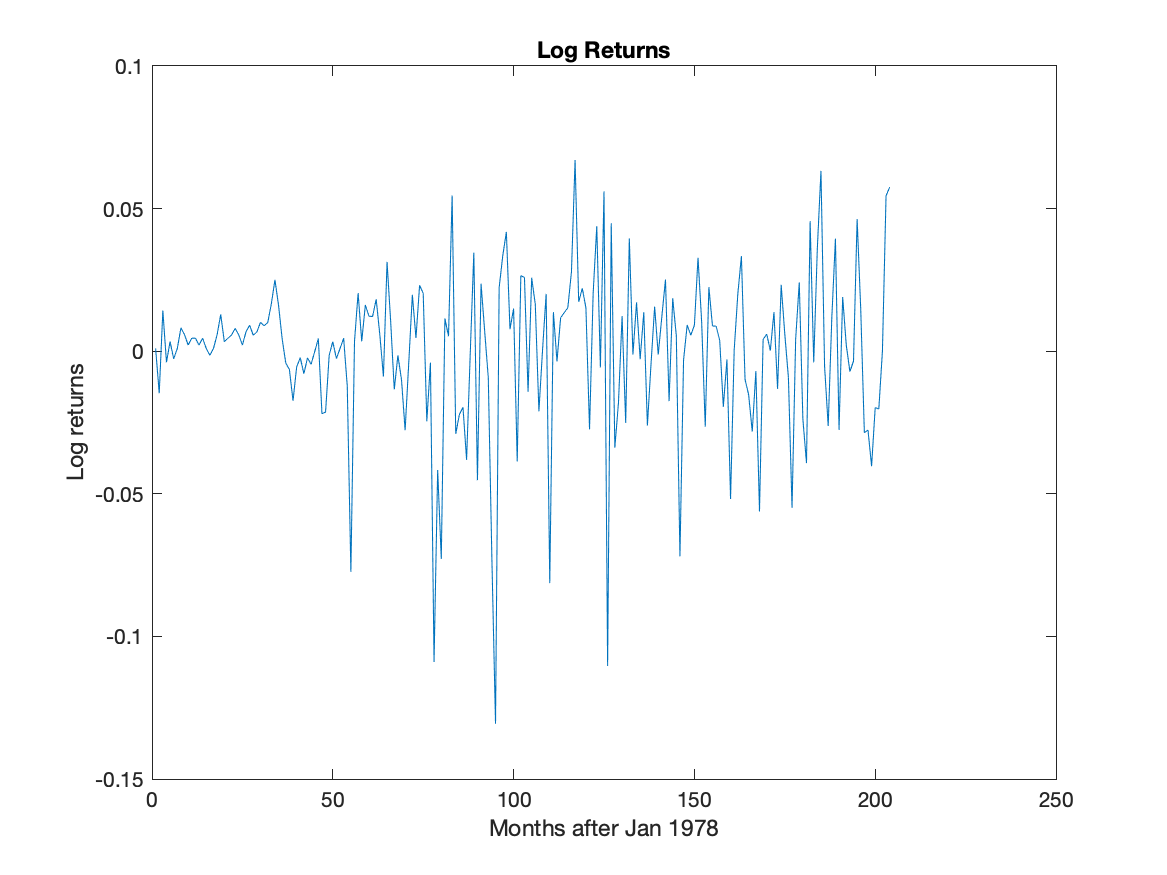
\includegraphics[width=8cm]{plots/log_returns.png}
\centering
\end{figure}

\section*{Problem 5}
\subsection*{Part a}
% Show expected value the same
\begin{align*}
    E[X_t] &= E[\cos(\omega t + Y)]\\
    &= E[\cos(\omega t) \cos(Y) - sin(\omega t) sin(Y)] && \text{Sum-difference for cos}\\
    &= \cos(\omega t) E[\cos(Y)] - sin(\omega t) E[sin(Y)]\\
    &= \text{TODO: Find dist. of cos(Y) and sin(Y)}
\end{align*}



\bibliographystyle{plain}
\bibliography{references}
\end{document}
